\section{Grundlagen des internen Rechnungswesens}

\textbf{Unterschied externes und internes Rechnungswesen}:
\begin{itemize}
	\item \textbf{externes Rechnungswesen}: Wenig detailliert, Gestaltung nach gesetzlichen Rechnungslegungsstandards, für externe Interessenten $\rightarrow$ Vergleichbarkeit zwischen Unternehmen
	\item \textbf{internes Rechnungswesen}: sehr detailliert, freie Gestaltung möglich, für interne Interessenten $\rightarrow$ interne Vergleichbarkeit
\end{itemize}

\textbf{Ziel vom internen Rechnungswesen}: Verteile Kosten auf die Produkttypen, Aufträge etc., um zu erkennen, welche Produkte, Aufträge, $\ldots$ gewinnbringend sind.\\

\textbf{Kalkulatorische Kosten}: Kosten, die im externen Rechnungswesen entweder in anderer Höhe (\textbf{Anderskosten}) oder gar nicht (\textbf{Zusatzkosten}) berücksichtigt werden.
\begin{itemize}
	\item \textbf{Beispiel}: kalkulatorische Zinsen für Sachanlagen, in denen nun auch Kosten des Eigenkapitals mit eingehen, obwohl man dafür \enquote{keine Rechnung erhält}
	\item Kosten Sachanlage = Abschreibungen + kalkulatorische Zinsen über den Buchwert
	\item \textbf{Annuitätenabschreibung}: Kosten Sachanlage in jeder Periode gleich
	\begin{tightcenter}
		$BW=C\cdot A+\cfrac{\text{Restwert}}{(1+r)^T}\qquad$, wobei $\qquad A=\cfrac{(1+r)^T-1}{r\cdot (1+r)^T}$
	\end{tightcenter}
	wobei $BW$: Anschaffungsbuchwert, $C=\text{Abschreibung}+ABS_t\;(\text{kalkulatorische Zinsen})$ und $r$: durchschnittliche Kosten von EK und FK. \textit{Bsp.s.FS4/6}
	\item \textbf{Wiederbeschaffungskosten}: Berücksichtigung, dass Vermögensgegenstände in Zukunft wegen steigenden Preisen teurer sind
	\begin{tightcenter}
		$\underbrace{EW}_\text{Mehrwert}=C\cdot A \iff C=\cfrac{EW}{A}\qquad$, wobei $\qquad A=\cfrac{(1+r)^T-1}{r}$
	\end{tightcenter}
	\textit{Bsp.s.FS4/7-8}
	\item \textbf{Geometrisch wachsende Abschreibungsbeträge}: zusätzliche Abschreibungen können auch anders über die Perioden verteilt sein
	\begin{tightcenter}
		$\underbrace{C_t}_\text{Abschreibung in Periode t}=\cfrac{EW}{T\cdot (1+r)^{T-t}}$
	\end{tightcenter}
	\textit{Bsp.s.FS4/9}
\end{itemize}
\bigskip

\textbf{Übersicht}:
\begin{center}
	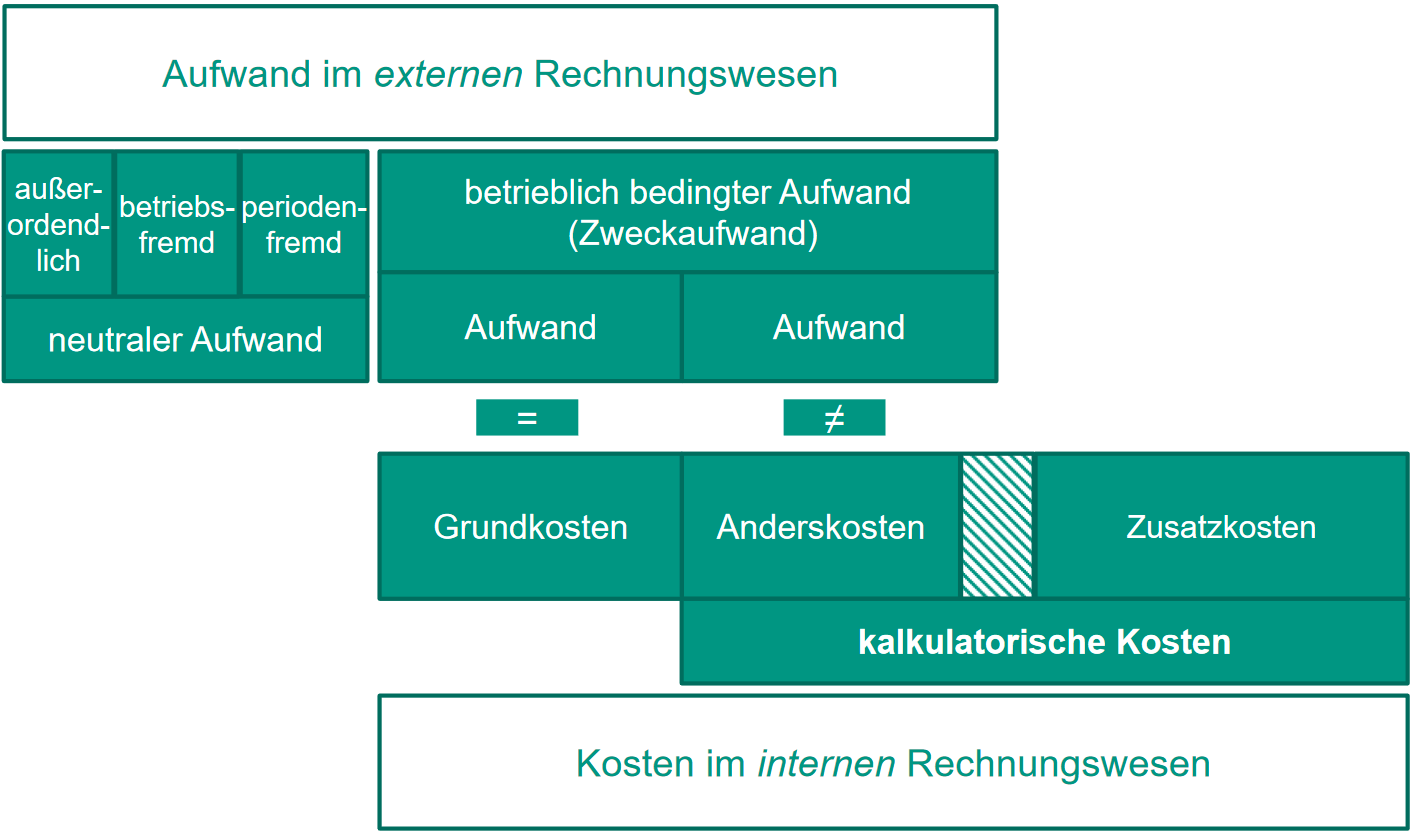
\includegraphics[width=0.7\textwidth]{images/kk-overview.png}
\end{center}
Beispiele:
\begin{itemize}
	\item außerordentlich: Katastrophenschäden
	\item betriebsfremd: Spenden für karitative Zwecke
	\item periodenfremd: Steuernachzahlung
\end{itemize}